\begin{figure*}[!t]
\centering

\begin{minipage}[t]{0.333\textwidth}
  \centering
  \vspace{0pt}
  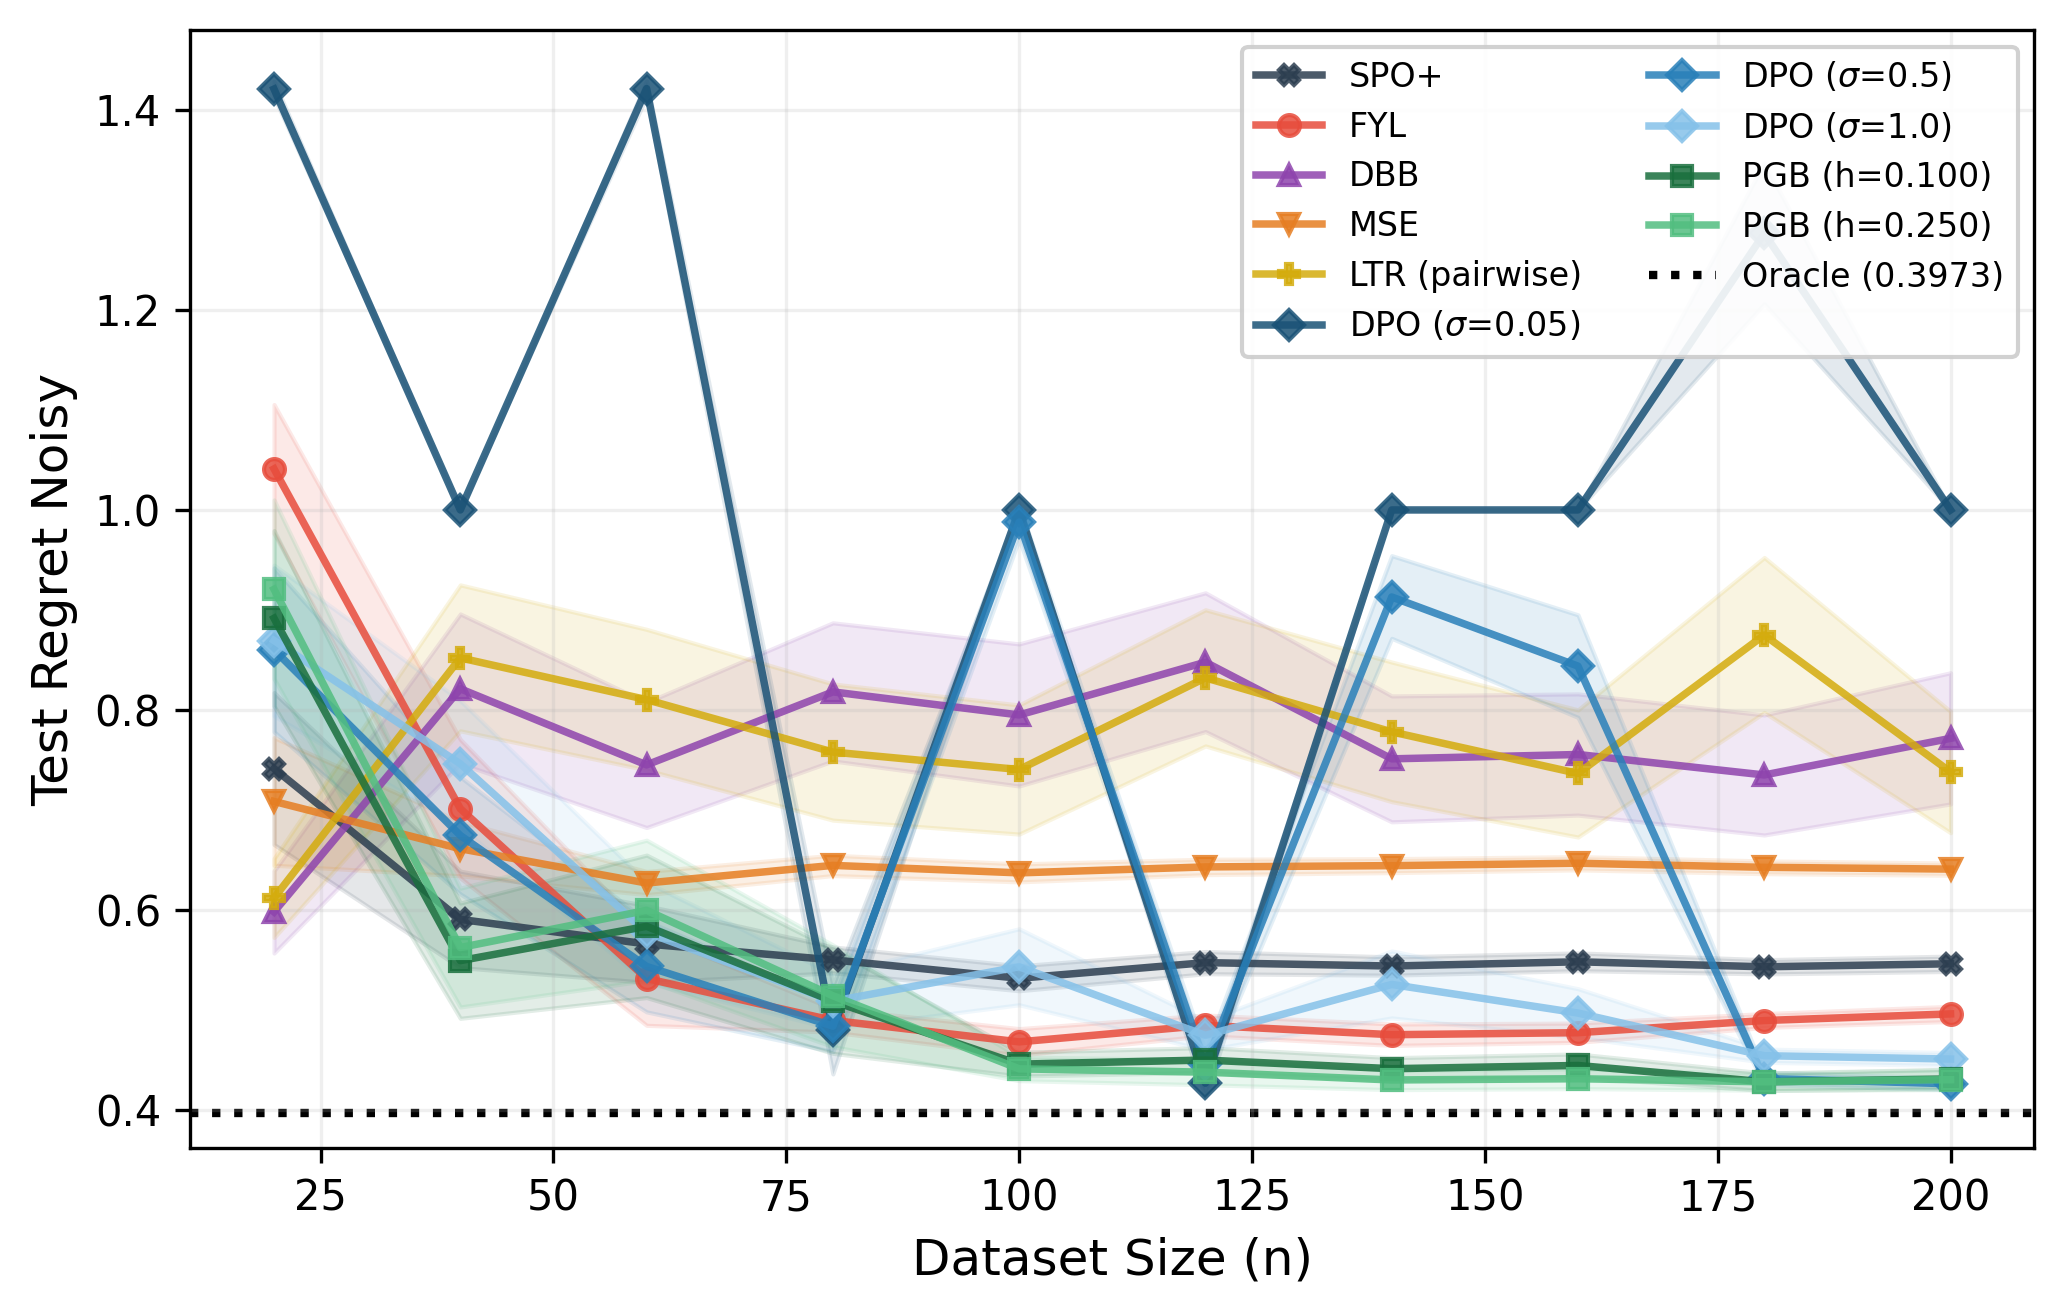
\includegraphics[width=\linewidth]{figures/regret_v3_noisy.png}
\end{minipage}%
\hfill%
\begin{minipage}[t]{0.33\textwidth}
  \centering
  \vspace{0pt}
  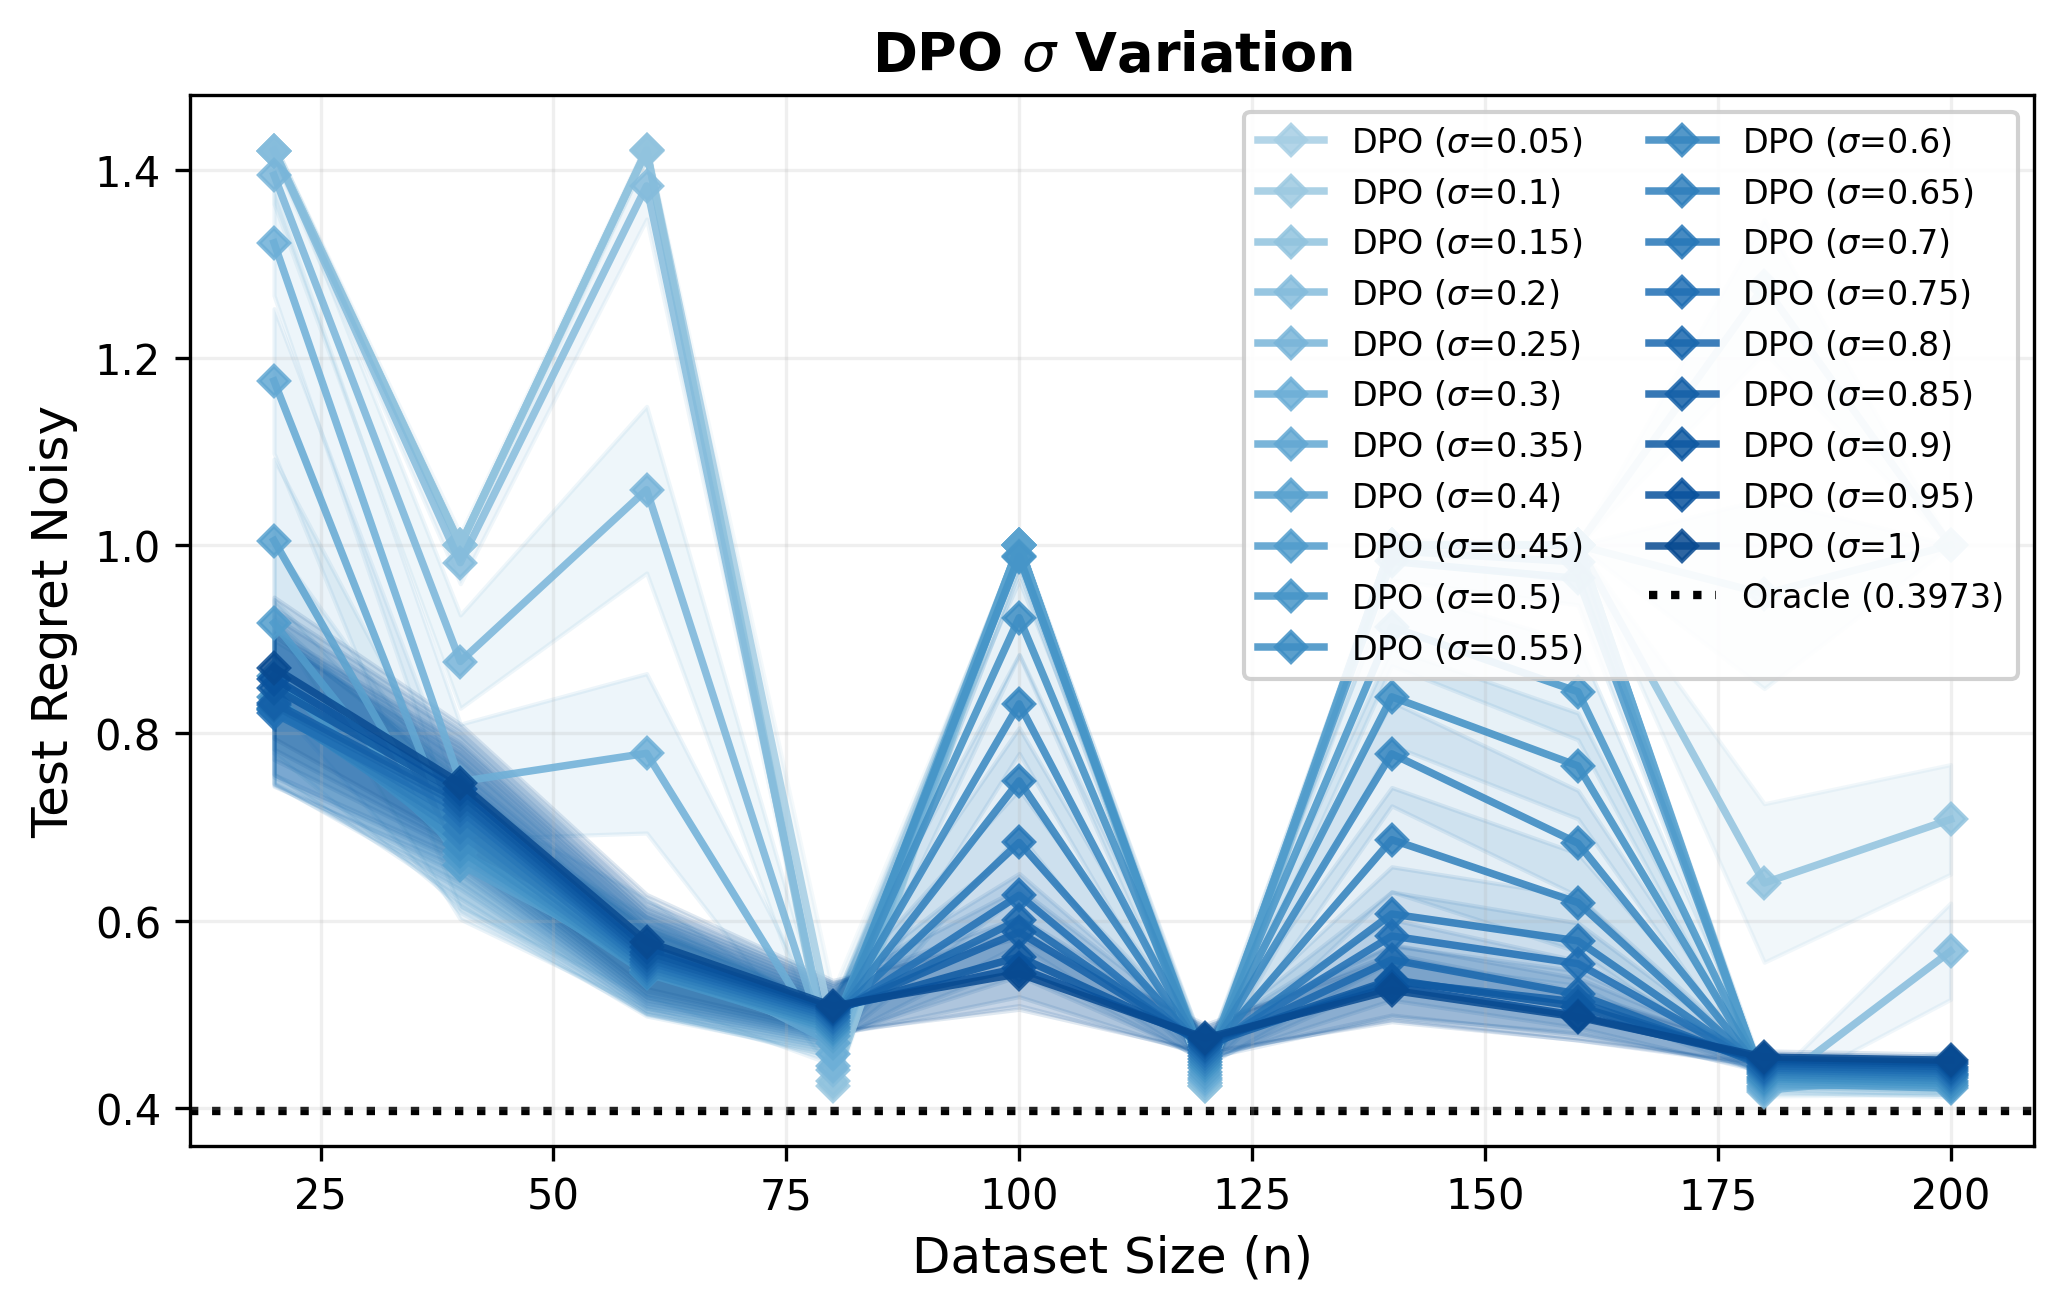
\includegraphics[width=\linewidth]{figures/regret_v3_noisy_dpo_sigma.png}
\end{minipage}%
\hfill%
\begin{minipage}[t]{0.33\textwidth}
  \centering
  \vspace{0pt}
  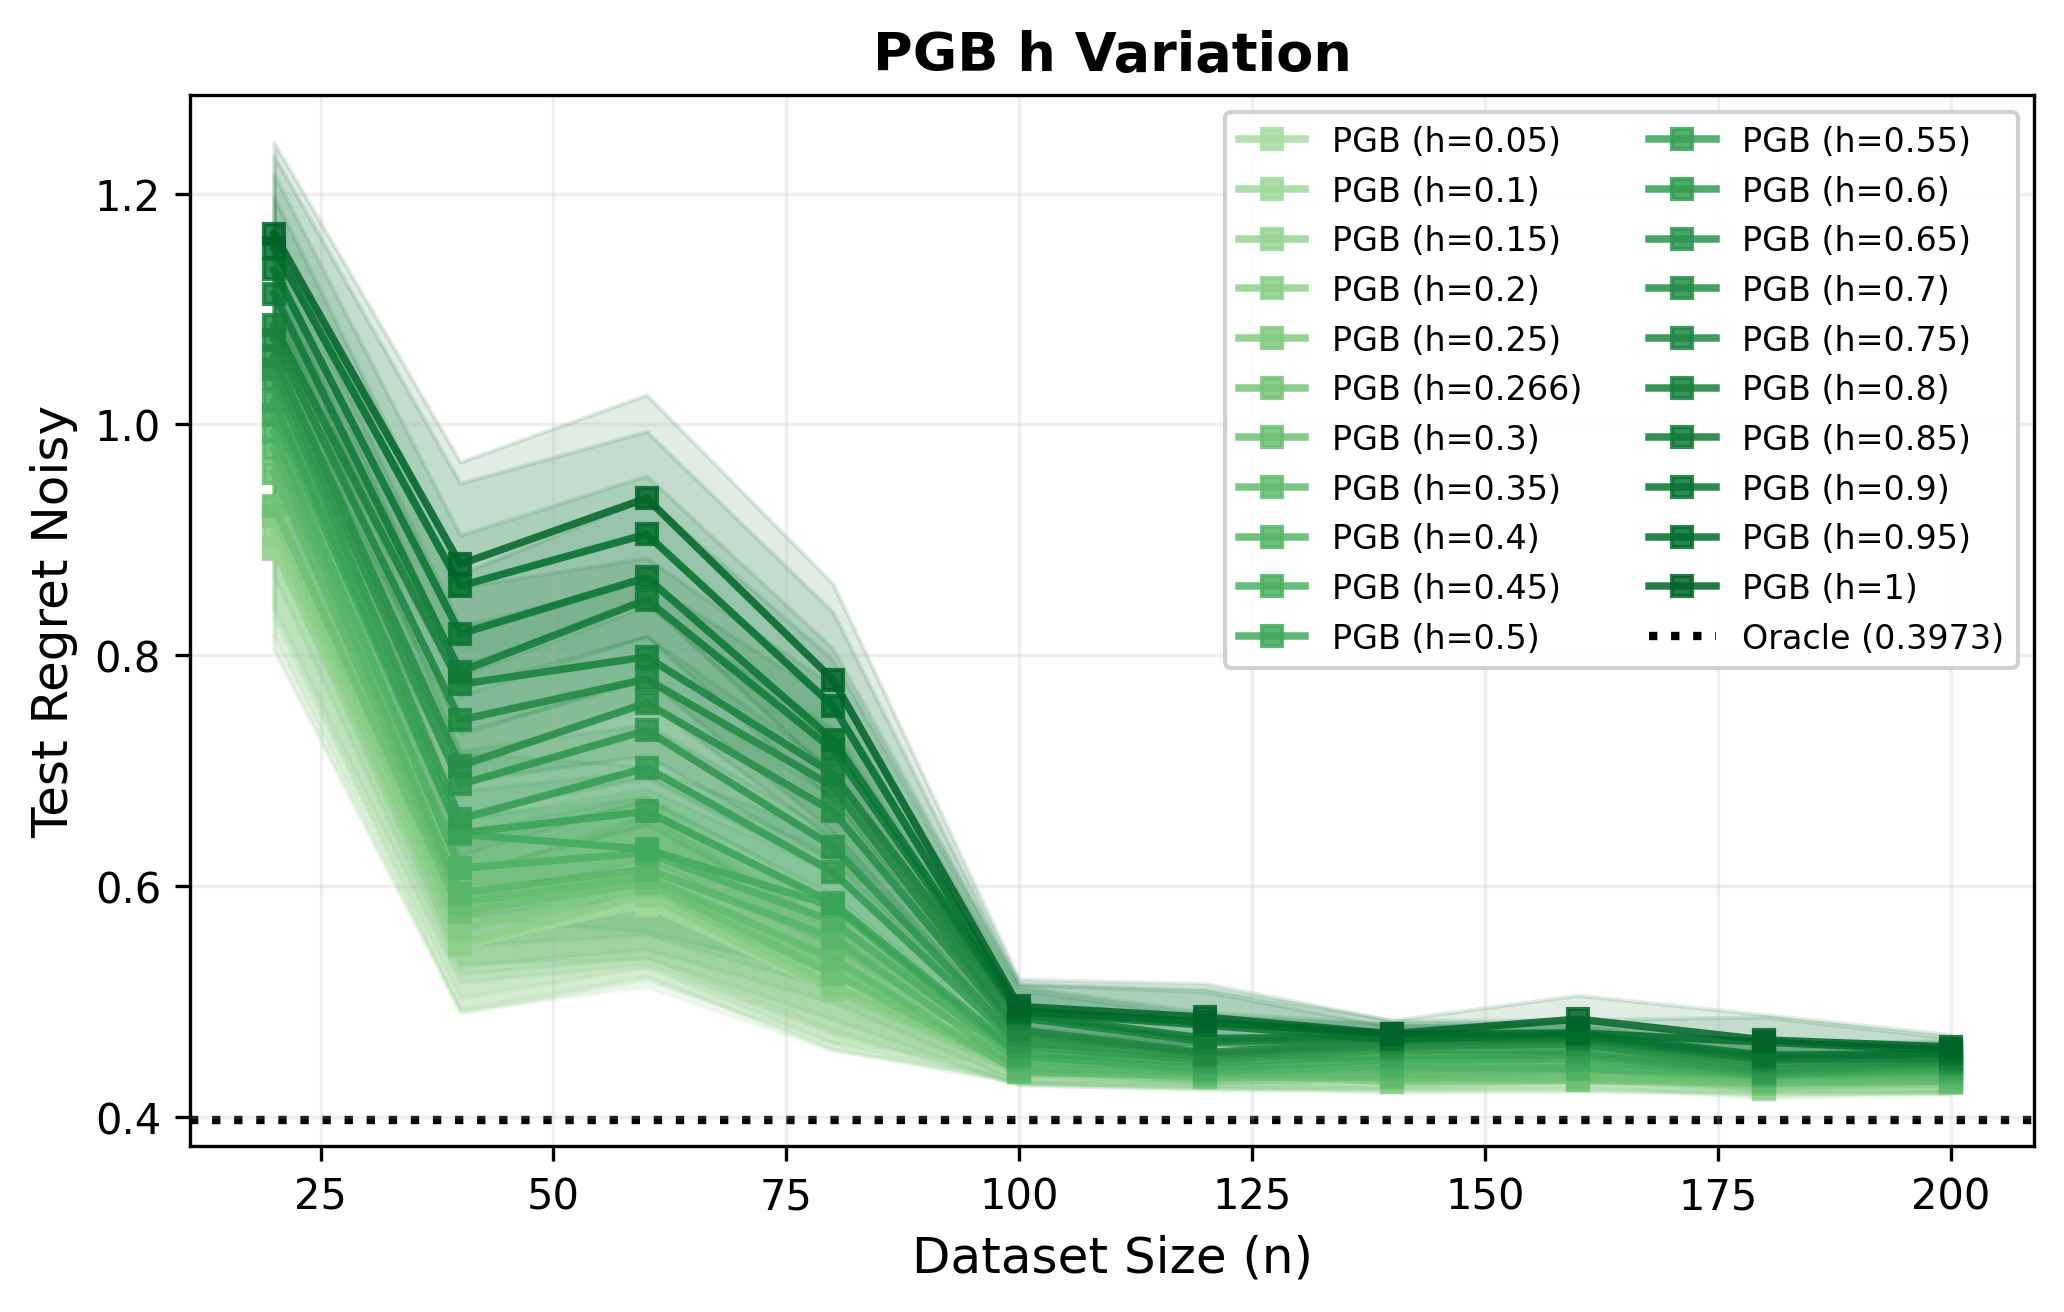
\includegraphics[width=\linewidth]{figures/regret_v3_noisy_pgb_h.png}
\end{minipage}

% Tighten gap between content and caption (local to this figure)
\vspace{-0.25em}
\setlength{\abovecaptionskip}{2pt}
\setlength{\belowcaptionskip}{0pt}

\caption[Impact of dataset size and hyperparameters on training of different decision-aware methods.]{\textbf{What solution is each method capable of learning?}
\textit{Left: }Here we train each objective at datasets of increasing size on the synthetic data task.
The dashed black line shows oracle decision regret. 
Only DPO and PG approach this optimal regret.
\textit{Center, Right:} Here we show how the DPO and PG training behavior changes as we vary key hyperparameters. 
DPO appears to struggle with too-low $\sigma$ values. Training is noisy and diverges for some dataset sizes.
 PG demonstrates faster convergence at lower $h$ values.
 }
%end caption
\label{fig:noisy_synth_regret}
\end{figure*}